\documentclass[fleqn]{article}

\usepackage{graphicx}
\usepackage{xurl}
\usepackage{url}
\usepackage{caption}
\usepackage{fancyhdr}
\usepackage{mathtools}
\usepackage{amsmath}
\usepackage{amssymb}
\usepackage{tikz}
\usepackage{listings}
\usepackage{xcolor}
\usepackage{float}

\definecolor{codegreen}{rgb}{0,0.6,0}
\definecolor{codegray}{rgb}{0.5,0.5,0.5}
\definecolor{codepurple}{rgb}{0.58,0,0.82}
\definecolor{backcolour}{rgb}{0.95,0.95,0.92}

\lstdefinestyle{mystyle}{
    backgroundcolor=\color{backcolour},   
    commentstyle=\color{codegreen},
    keywordstyle=\color{magenta},
    numberstyle=\tiny\color{codegray},
    stringstyle=\color{codepurple},
    basicstyle=\ttfamily\footnotesize,
    breakatwhitespace=false,         
    breaklines=true,                 
    captionpos=b,                    
    keepspaces=true,                 
    numbers=left,                    
    numbersep=5pt,                  
    showspaces=false,                
    showstringspaces=false,
    showtabs=false,                  
    tabsize=2
}

\lstset{style=mystyle}

\usepackage{xepersian}

\settextfont[BoldFont={XB Zar bold.ttf}]{XB Zar.ttf}
\setlength\parindent{0pt}



\newcommand{\expnumber}{سوم}



\title{

\includegraphics[width=0.4\textwidth]{sharif.png}\\
\normalsize{دانشکده مهندسی کامپیوتر}\\
\vspace{1cm}
    
\huge{آزمایشگاه معماری کامپیوتر}
\\ \vspace{.8cm}
\Large{گزارش آزمایش \expnumber}
\\ \vspace{.8cm}
\Large{عنوان آزمایش : جمع/تفریق کننده ممیز شناور}
}

\author{
\\
دکتر حمید سربازی آزاد
\\ \vspace{.4cm}
\\
  سارا آذرنوش       ---      98170668
\\ \vspace{0.2cm} \\
  کسری امانی       ---      98101171
\\ \vspace{0.2cm} \\
  پارسا محمدیان       ---      98102284
\\ \vspace{.4cm}
}

\date{\today}

\begin{document}

\clearpage\maketitle
\thispagestyle{empty}

\newpage

\pagestyle{fancy}
\lhead{آزمایشگاه معماری کامپیوتر}

\rhead{آزمایش \expnumber}

\tableofcontents

\setcounter{page}{1}

\newpage

\section{مقدمه}
در کامپیوتر برای ذخیره اعداد اعشاری از استاندارد 
\lr{IEEE 754}
استفاده می‌شود. این استاندارد عدد را به نماد علمی تبدیل می‌کند سپس مانتیس و نما و علامت عدد را دخیره می‌کند. 
البته تمام این‌ها در مبنای دو اتفاق می‌افتد.

\section{هدف آزمایش}
در این آزمایش قصد داریم یک جمع/تفریق کننده ممیز شناور 12 بیتی شبیه به استاندارد 
\lr{IEEE 754}
طراحی کنیم.

\section{شرح آزمایش}
همانطور که در مقدمه گفته شد این استاندارد از نمایش نماد علمی استفاده می‌کند. برای جمع و تفریق اعداد 
در این نمایش ابتدا باید نما را یکسان کنیم. در مبنای دو این کار را با افزایش نماد کوچکتر و متناظرا شیفت دادن مانتیس 
آن به راست انجام می‌دهیم. پس از آن عملیات جمع یا تفریق را بر روی مانتیس انجام می‌دهیم. البته در استاندارد 
\lr{IEEE 754}
برای صرفه‌جویی در بیت‌ها، تک رقم سمت چپ ممیز یک فرض می‌شود. پس برای تولید خروجی باید حاصل جمع یا تفریق را 
به فرم نرمال دربیاوریم. 

در ابتدا مراحل را در 
\lr{ASM}
طراحی میکنیم و سپس با توجه به استیت ها پیش میرویم. شکل نمودار 
\lr{ASM}
در تصویر 
\ref{asm}
قابل مشاهده است.

\begin{figure}[!htbp]
    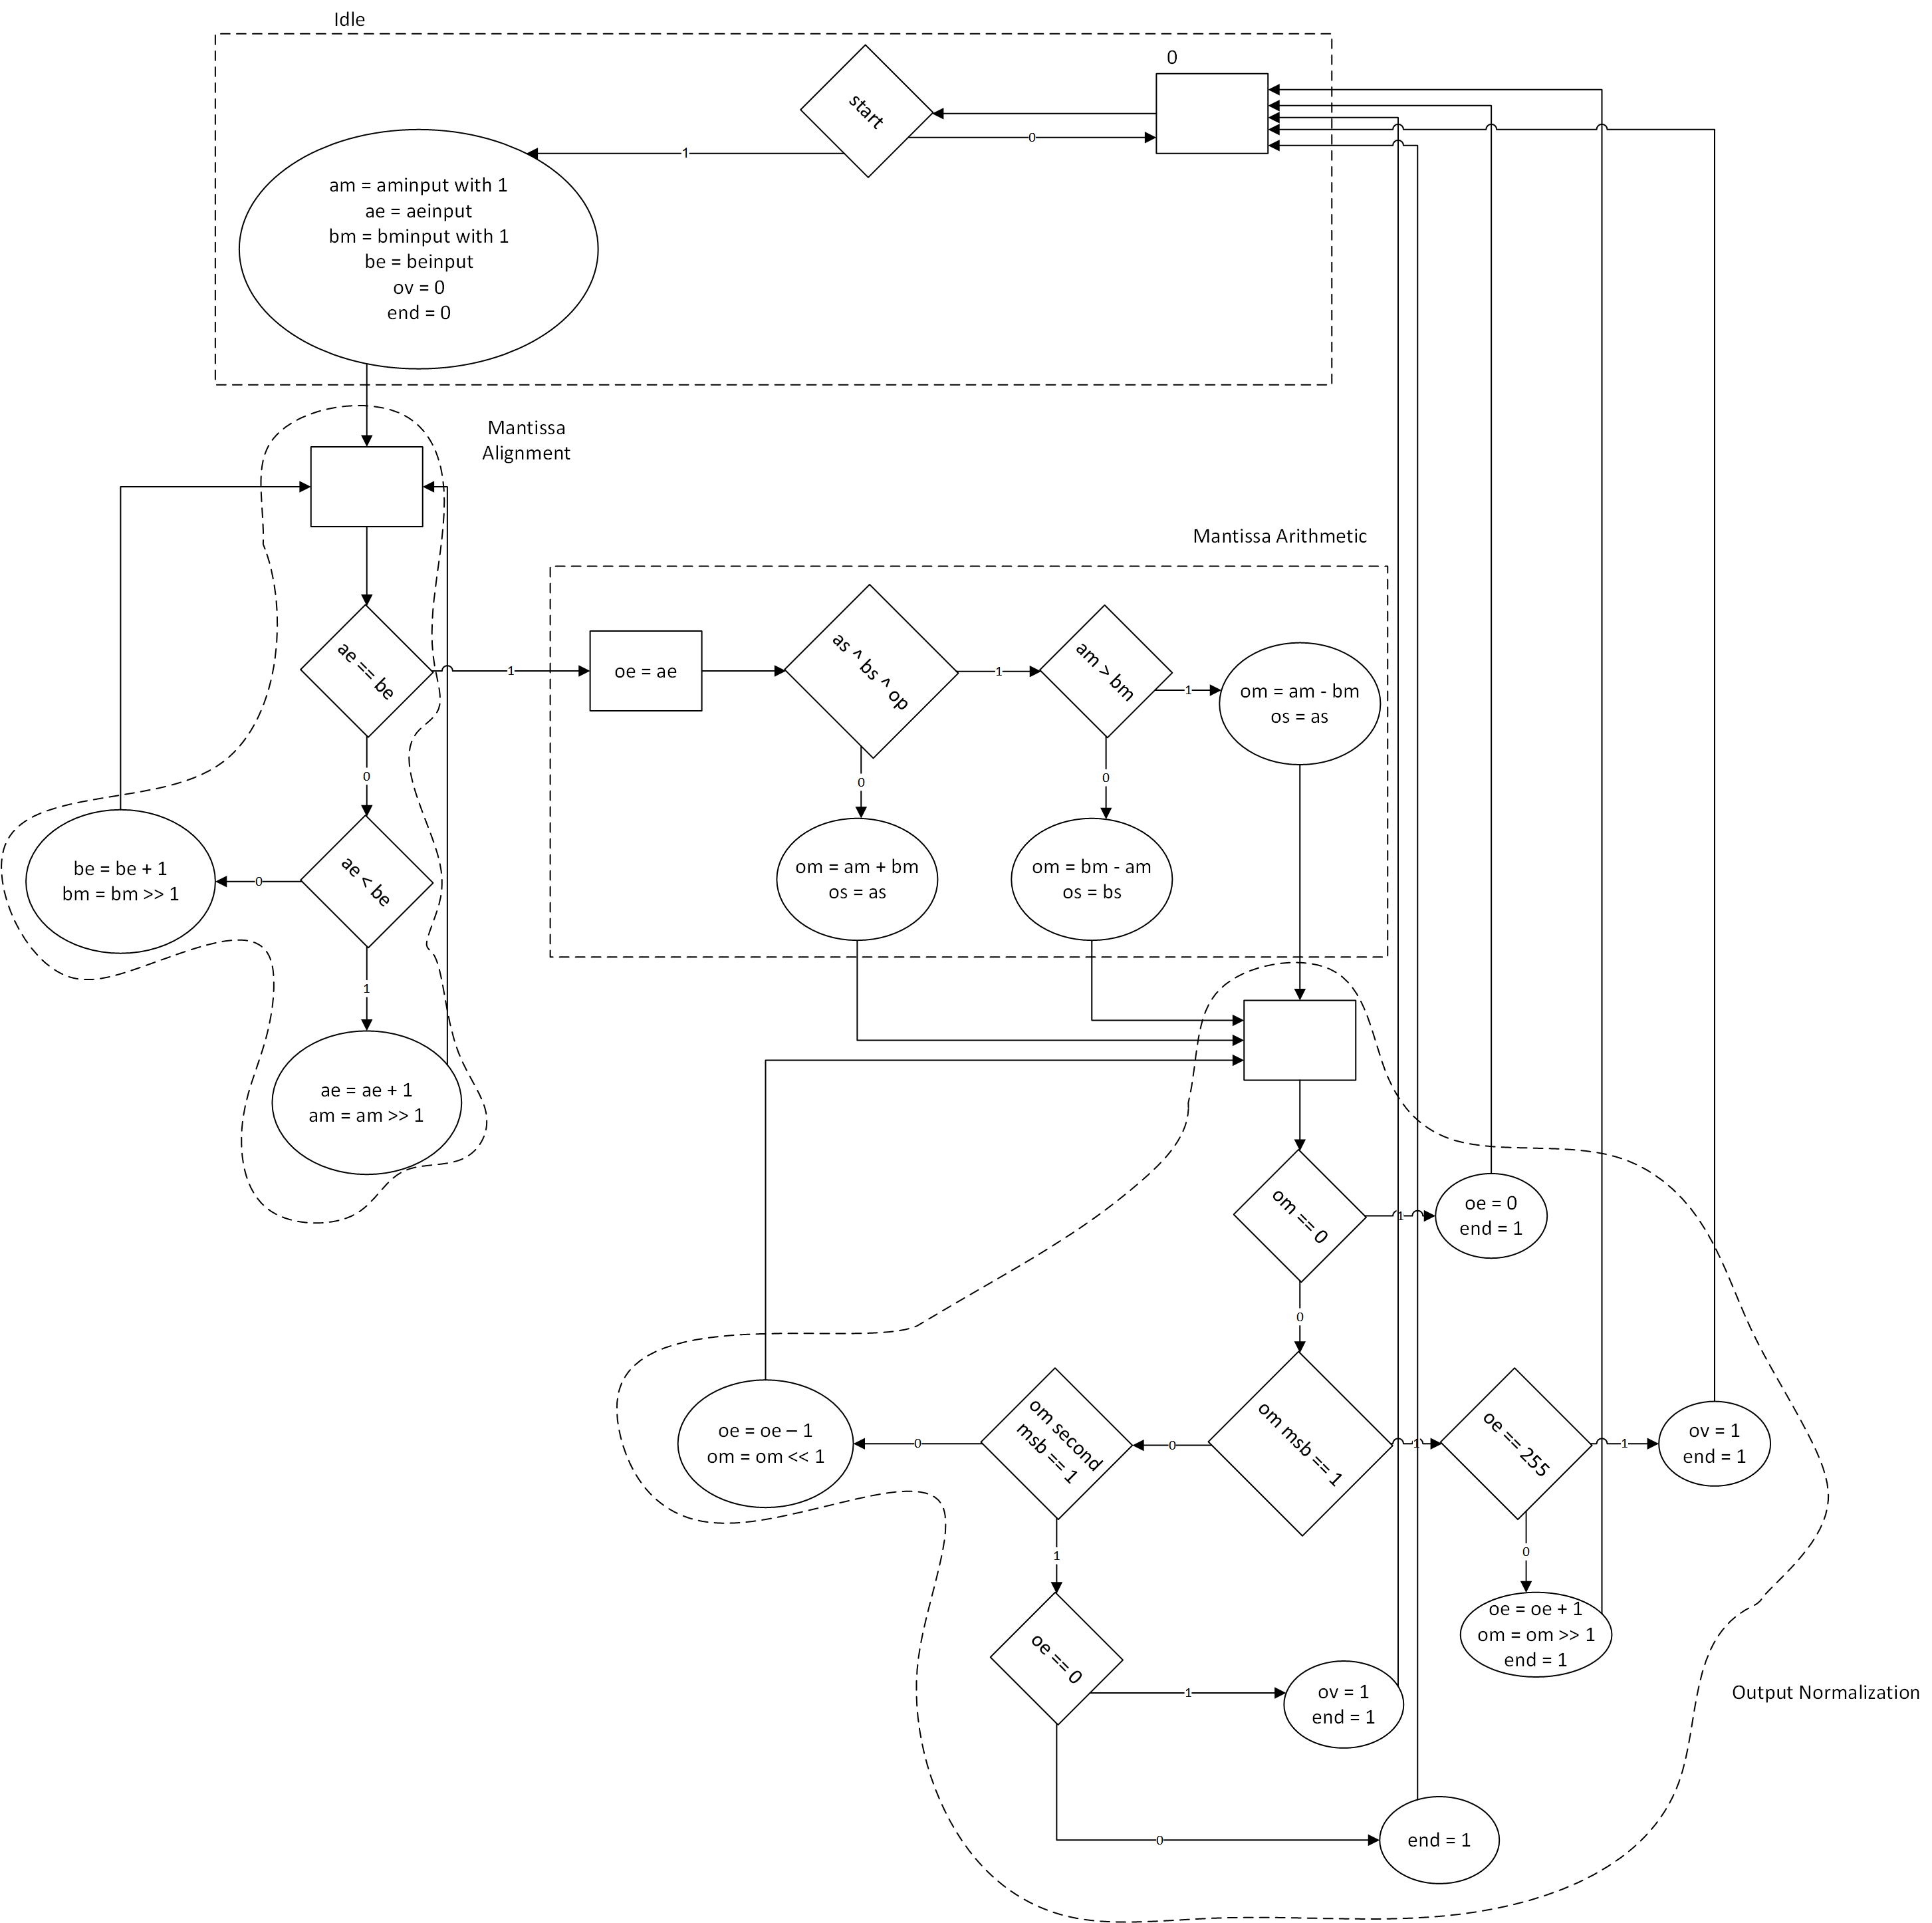
\includegraphics[width=\textwidth]{Assets/ASM.png}
    \caption{نمودار \lr{ASM}}
    \label{asm}
\end{figure}

با توجه به گفته دستورکار از شمارنده استفاده میکنیم و  اکسپوننت های دو عدد را مقایسه میکنیم هر کدام که کوچک تر بود آن را شیفت داده و به مانتیس آن اضافه میکنیم تا زمانی که برابر شوند و وارد یک ماکس 8 بیتی میشوند که ترتیب ورودی جمع/تفریق کننده 8 بیتی باینری را برای تفریق مشخص میکنند(عدد با مانتیس کوچکتر از عدد با مانتیس بزرگتر کم میشود.)

نمودار حالت در شکل 
\ref{sd}
آمده است. 

\begin{figure}[!htbp]
    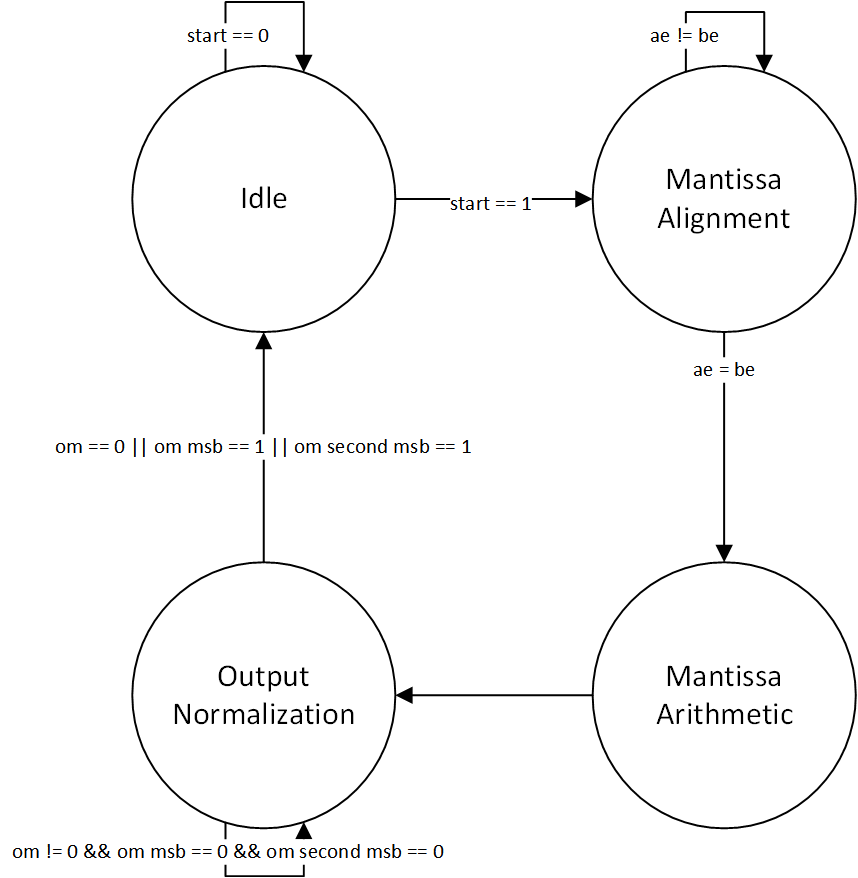
\includegraphics[width=\textwidth]{Assets/StateDiagram.png}
    \caption{نمودار حالت}
    \label{sd}
\end{figure}

استیت ها به شکل زیر تغییر میکنند

چک کردن اکسپوننت و افزودن به آن با مقایسه کننده و شمارنده

شیفت مانتیس ها و ماکس برای ترتیب تفریق کننده و شونده

جمع و تفریق مانتیس و لود آن

مقایسه مانتیس ها برای انتخاب در ماکس

در آخر با پیاده‌سازی واحد کنترل و مسیر داده مدار را پیاده سازی می‌کنیم.


\section{نتیجه آزمایش}
یک جمع/تفریق کننده ممیز شناور داریم که با سیگنال 
\lr{start}
شروع به کار می‌کند و دو عدد داده شده را جمع می‌کند. پس از پایان عملیات سیگنال 
\lr{end}
که نشانگر پایان عملیات است 1 می‌شود. اگه هنگام انجام عملیات سرریز رخ داده باشد نیز سیگنال 
\lr{ov}
فعال می‌شود. 

در آخر برای تست مدار مقادیر مختلف را جمع/تفریق می‌کنیم. نمونه‌های از خروجی در اشکال 
\ref{t1}
\ref{t2}
\ref{t3}
\ref{t4}
\ref{t5}
آمده است.

\textbf{دقت شود که کلید استارت باید انقد نگه داشته شود تا مقدار عدد در رجیسترها لود شود. (حداقل یک کلاک)}

\begin{figure}[!htbp]
    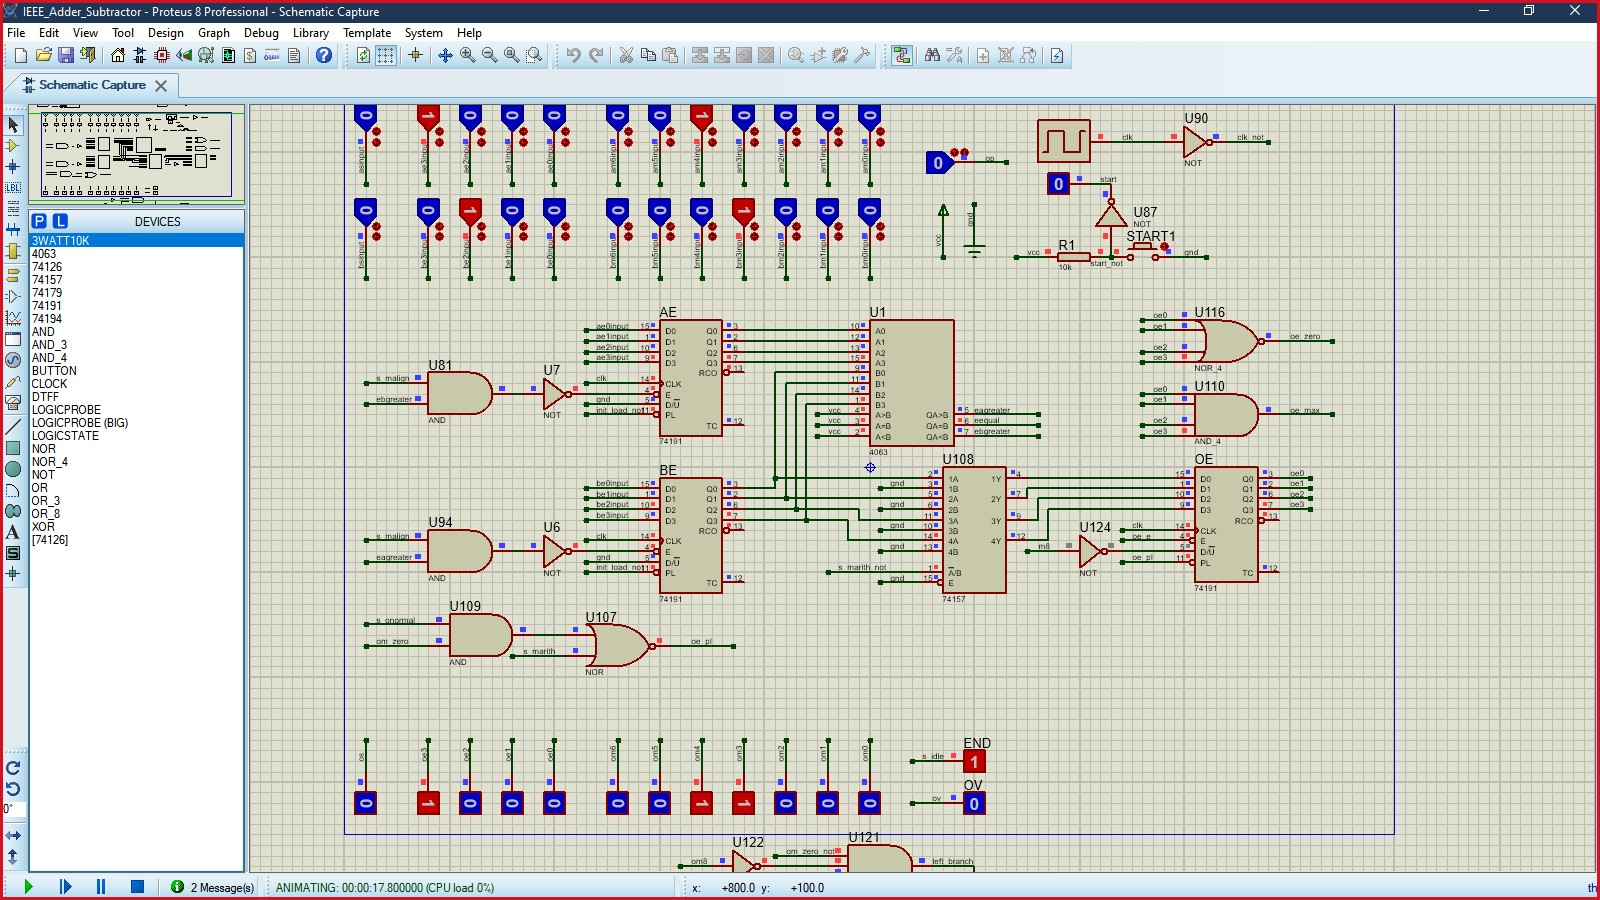
\includegraphics[width=\textwidth]{Assets/test1.jpg}
    \caption{تست اول - جمع ساده}
    \label{t1}
\end{figure}

\begin{figure}[!htbp]
    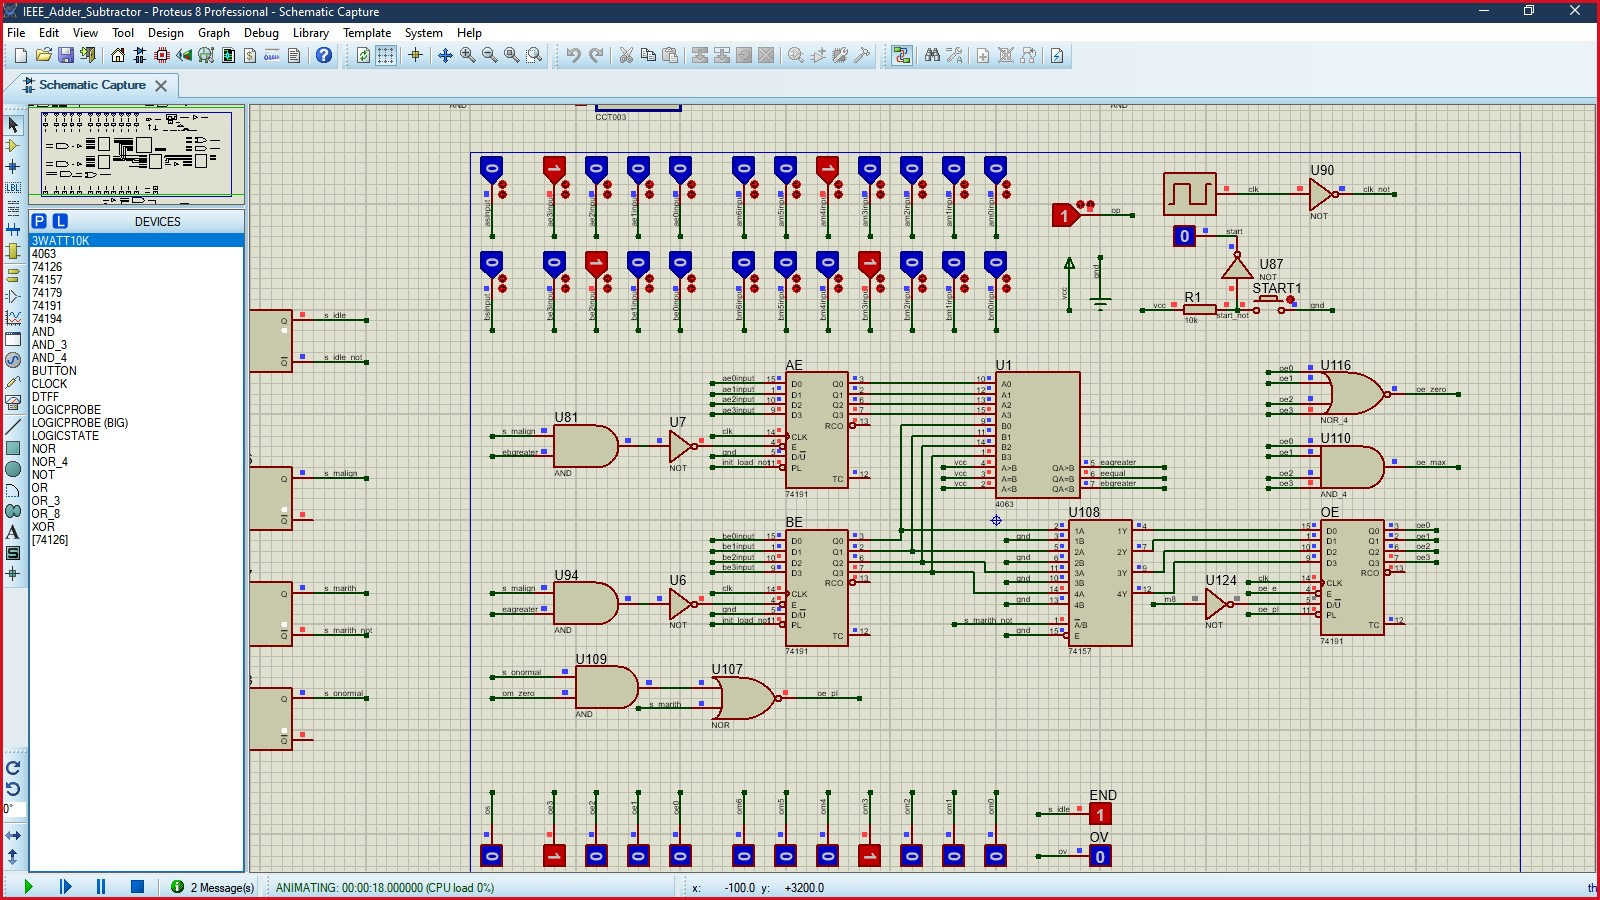
\includegraphics[width=\textwidth]{Assets/test2.jpg}
    \caption{تست 2 - تفریق ساده}
    \label{t2}
\end{figure}

\begin{figure}[!htbp]
    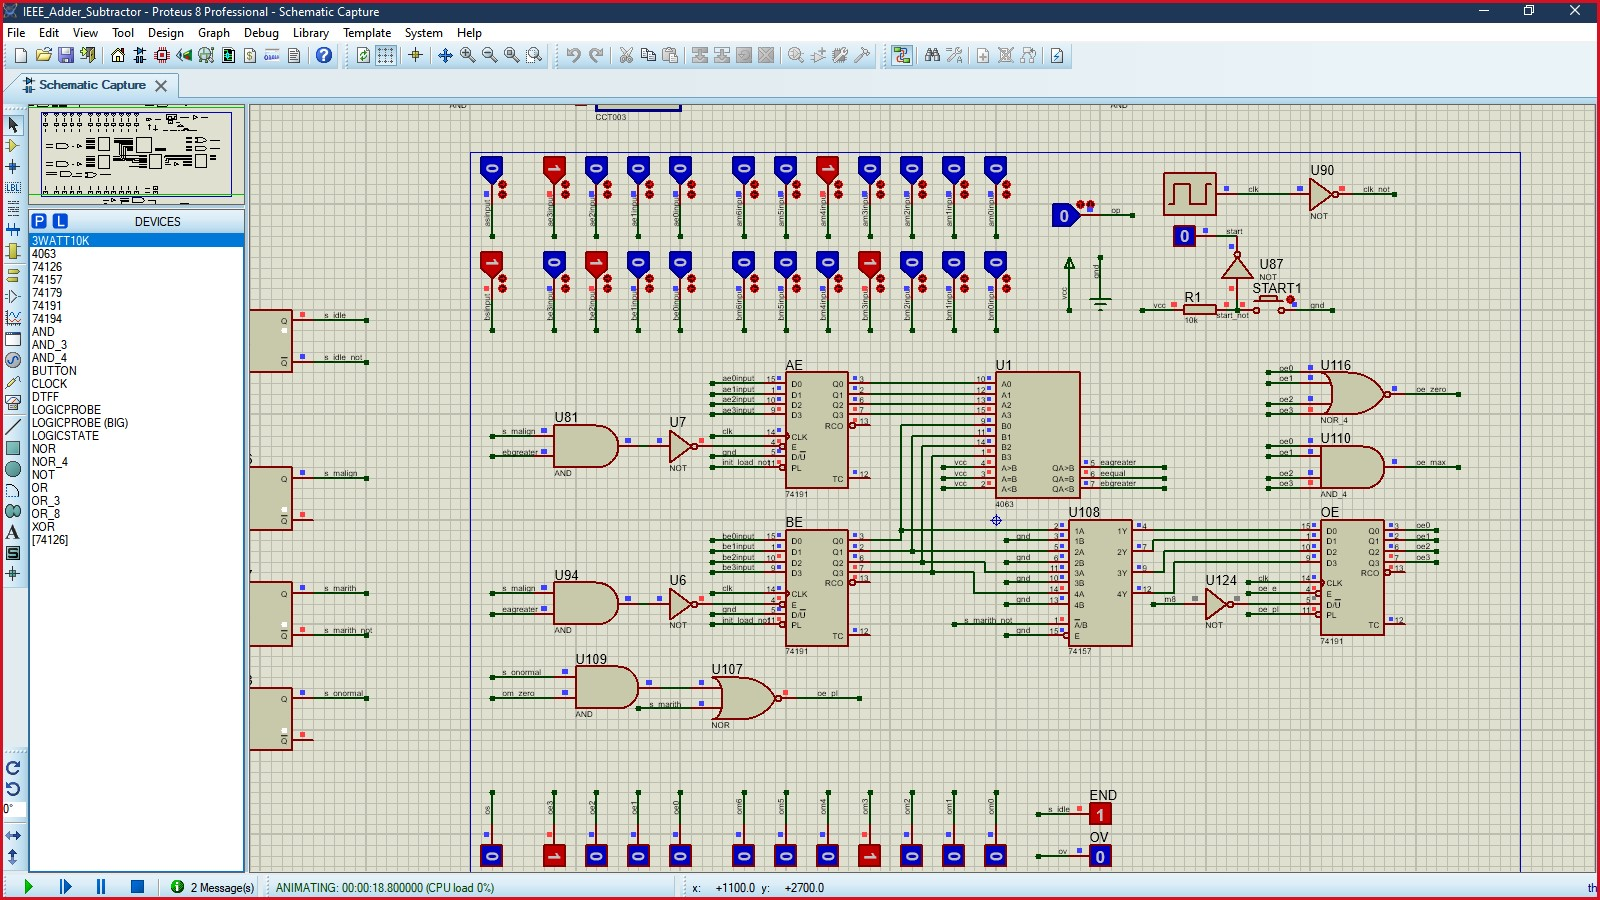
\includegraphics[width=\textwidth]{Assets/test3.jpg}
    \caption{تست 3 - جمع با عدد منفی}
    \label{t3}
\end{figure}

\begin{figure}[!htbp]
    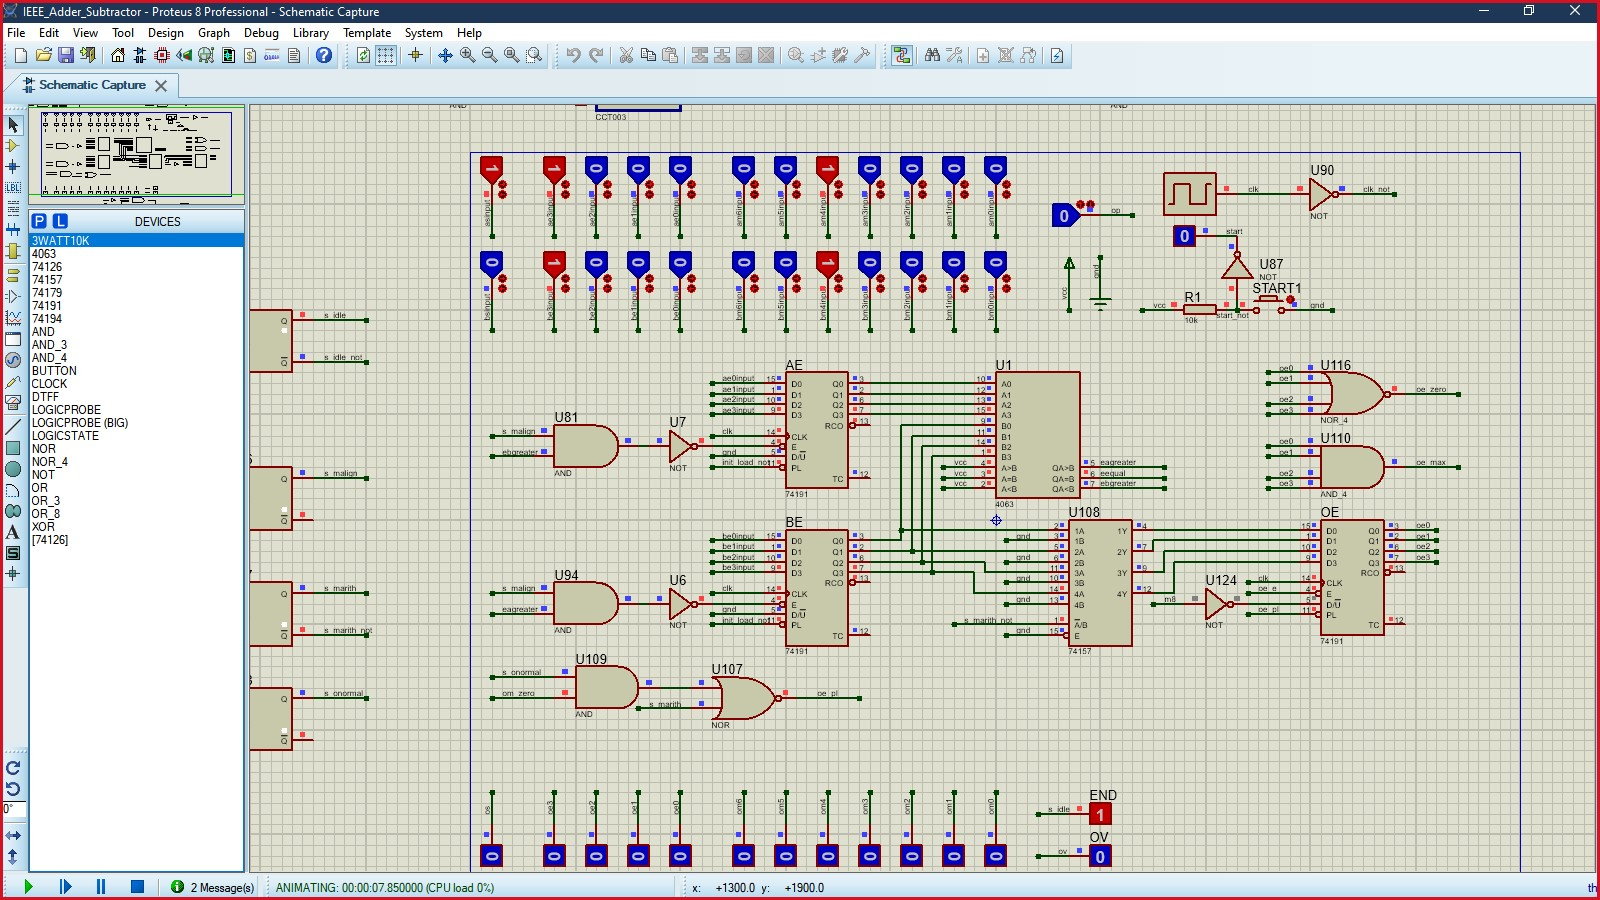
\includegraphics[width=\textwidth]{Assets/test4.jpg}
    \caption{تست 4 - یک عدد منهای خودش (حاصل صفر که باید نرمال شود)}
    \label{t4}
\end{figure}

\begin{figure}[!htbp]
    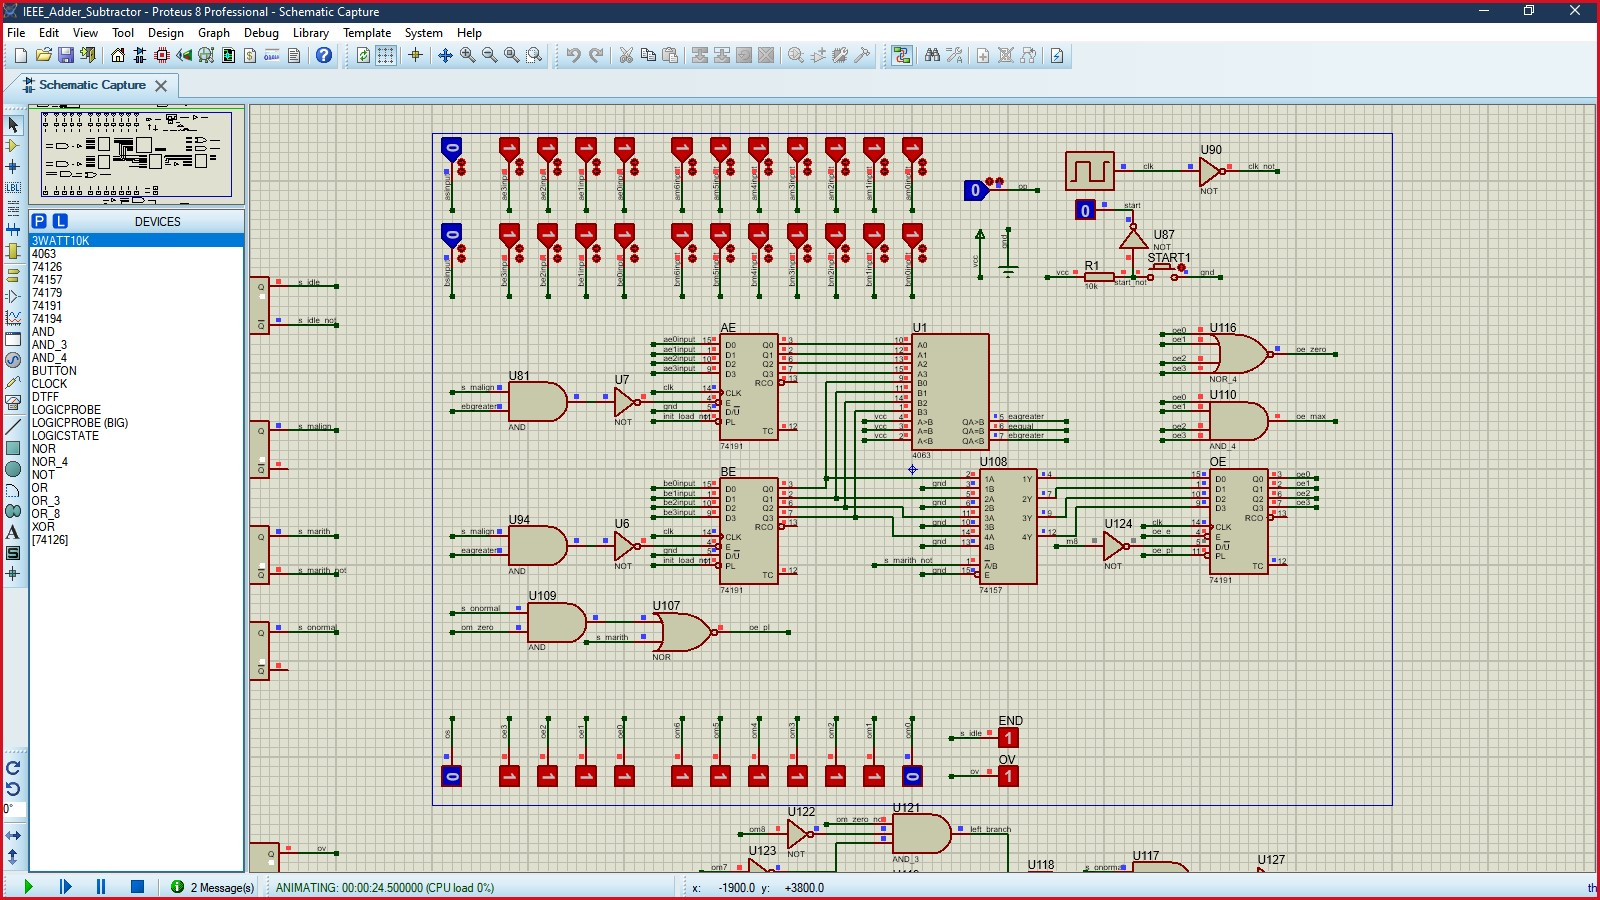
\includegraphics[width=\textwidth]{Assets/test5.jpg}
    \caption{تست 5 - سرریز}
    \label{t5}
\end{figure}




\end{document}